Welcome to the first assignment! During this assignment, you will practice your
math skills in an environment more similar to the one that you will face during
the course assessment. Although the questions will not be the same, they will
follow the same structure and you will have to solve the exercises using the
Dirac notation or matrix--vector multiplication.

Together with this assignment, you will find the \LaTeX { template} for you to use
when solving the exercises and writing down your answers. Remember to upload a
single pdf file with the full development of the assignment and the answers.

\begin{question}
Given the quantum state $\ket{\psi} = \sqrt{\frac{1}{3}} \ket{0} + \sqrt{\frac{2}{3}} \ket{1}$. Is $\ket{\psi}$ a valid quantum state? Explain why.
\label{qst:assignment1_1}
\end{question}
{\small
\texttt{Write down your solution here:}
\begin{equation*}
  \begin{split}
    \sqrt \frac{1}{3} \ket{0} + \sqrt \frac{2}{3} \ket{1} = \frac{1}{3} \ket{0} + \frac{2}{3} \ket{1} = 1
  \end{split}
\end{equation*}}
\vspace{0.1cm}

\begin{question}
Given the quantum states $\ket{\psi_{1}} = \frac{3}{5} \ket{0} + \frac{4}{5} \ket{1}$ and $\ket{\psi_{2}} = \frac{3}{5} \ket{0} - \frac{4}{5} \ket{1}$. What is the resulting quantum state $\ket{\psi} = \ket{\psi_{2}} - \ket{\psi_{1}}$?
\label{qst:assignment1_2}
\end{question}
{\small
\texttt{Write down your solution here:}
\begin{equation*}
\begin{split}
    \ket{\psi} &= (\sqrt{\tfrac{3}{5}}\ket{0}-\sqrt{\tfrac{4}{5}}\ket{1})
    - (\sqrt{\tfrac{3}{5}}\ket{0}+\sqrt{\tfrac{4}{5}}\ket{1}) \\
    \ket{\psi} &= (\sqrt{\tfrac{3}{5}}\ket{0}-\sqrt{\tfrac{4}{5}}\ket{1})
    - (\sqrt{\tfrac{3}{5}}\ket{0}-\sqrt{\tfrac{4}{5}}\ket{1}) \\
    \ket{\psi} &= \sqrt{\tfrac{3}{5}}\ket{0}-\sqrt{\tfrac{4}{5}}\ket{1}
    - \sqrt{\tfrac{3}{5}}\ket{0}-\sqrt{\tfrac{4}{5}}\ket{1}\\
    \ket{\psi} &= -\tfrac{4}{5}\ket{1}-\tfrac{4}{5}\ket{1}=-\tfrac{8}{5}\ket{1}=-1\tfrac{3}{5}\ket{1}\\
    \ket{\psi} &= -1\tfrac{3}{5}\ket{1} = \frac{-1\tfrac{3}{5}\ket{1}}{1\frac{3}{5}} = -\ket{1}
\end{split}
\end{equation*}}
\vspace{0.1cm}

\begin{question}
Assume that you can only use the quantum gates from the set $\mathcal{Q} = \left\lbrace I,\,X,\,Y,\,Z,\,H\right\rbrace$. Is it possible to create the quantum state $\ket{\psi_{out}} = \frac{i}{\sqrt{2}} \ket{0} - \frac{i}{\sqrt{2}} \ket{1}$ starting from the qubit $\ket{\psi_{in}} = \ket{0}$. Explain how?
\label{qst:assignment1_3}
\end{question}
{\small
\texttt{Write down your solution here:}
\begin{equation*}
  \begin{split}
  \ket{\psi_{out}}=\tfrac{i}{\sqrt{2}}\ket{0}-\tfrac{i}{\sqrt{2}}\ket{1} = \\
  \ket{\psi_{out}}=i(\tfrac{1}{\sqrt{2}}\ket{0}-\tfrac{1}{\sqrt{2}}\ket{1}) = \\
  \ket{\psi_{out}}=\tfrac{1}{\sqrt{2}}(\ket{0}-\ket{1}) \\
  \\
  \ket{\phi}=\tfrac{1}{\sqrt{2}}(\ket{0}-\ket{1}) \\
  H\ket{0} = \tfrac{1}{\sqrt{2}}(\ket{0}+\ket{1}) \\
  ZH=Z(\tfrac{1}{\sqrt{2}}(\ket{0}+\ket{1})=\tfrac{1}{\sqrt{2}}(\ket{0}-\ket{1})
  \end{split}
\end{equation*}}
\vspace{0.1cm}

\begin{question}
Assume that you can only use the quantum gates from the set $\mathcal{Q} = \left\lbrace I,\,X,\,Y,\,Z,\,H\right\rbrace$. Is it possible to create the quantum state $\ket{\psi_{out}} = \frac{1}{\sqrt{2}} \ket{0} + \frac{i}{\sqrt{2}} \ket{1}$ starting from the qubit $\ket{\psi_{in}} = \ket{0}$. Explain how?
\label{qst:assignment1_4}
\end{question}
{\small
\texttt{Write down your solution here:}
\texttt{The only way to achieve $-\ket{1}$ is by applying a gate S, which is not allowed to be used , thus not possible. Since the only gate that uses imaginary numbers is Y, Y flips the basis states.}
\begin{equation*}
  \begin{split}
  \ket{\psi_{out}}=\tfrac{1}{\sqrt{2}}(\ket{0}+i\ket{1})= \\
  H\ket{0}=\tfrac{1}{\sqrt{2}}(\ket{0}+\ket{1}) \\
  \\
  \ket{0} \rightarrow \ket{0}, \ket{1} \rightarrow -\ket{1}
  \end{split}
\end{equation*}}
\vspace{0.1cm}

\begin{question}
What state does the $S$ gate transform the quantum state $\ket{-i}$ into?
\label{qst:assignment1_5}
\end{question}
{\small
\texttt{Write down your solution here:}
\begin{equation*}
  \begin{split}
    \ket{\psi} &= S \ket{-i} =
    \begin{pmatrix}
        1 & 0 \\ 0 & i
    \end{pmatrix}
    \cdot
    \frac{1}{\sqrt{2}}
    \begin{pmatrix}
        1 \\ -i
    \end{pmatrix}
    =
    \frac{1}{\sqrt{2}}
    \begin{pmatrix}
        1 \\ i & (-i)
    \end{pmatrix}
    =
    \frac{1}{\sqrt{2}}
    \begin{pmatrix}
        1 \\ 1
    \end{pmatrix}
    =
    \ket{+}
  \end{split}
\end{equation*}}
\vspace{0.1cm}

\begin{figure}[t]
  \centerline{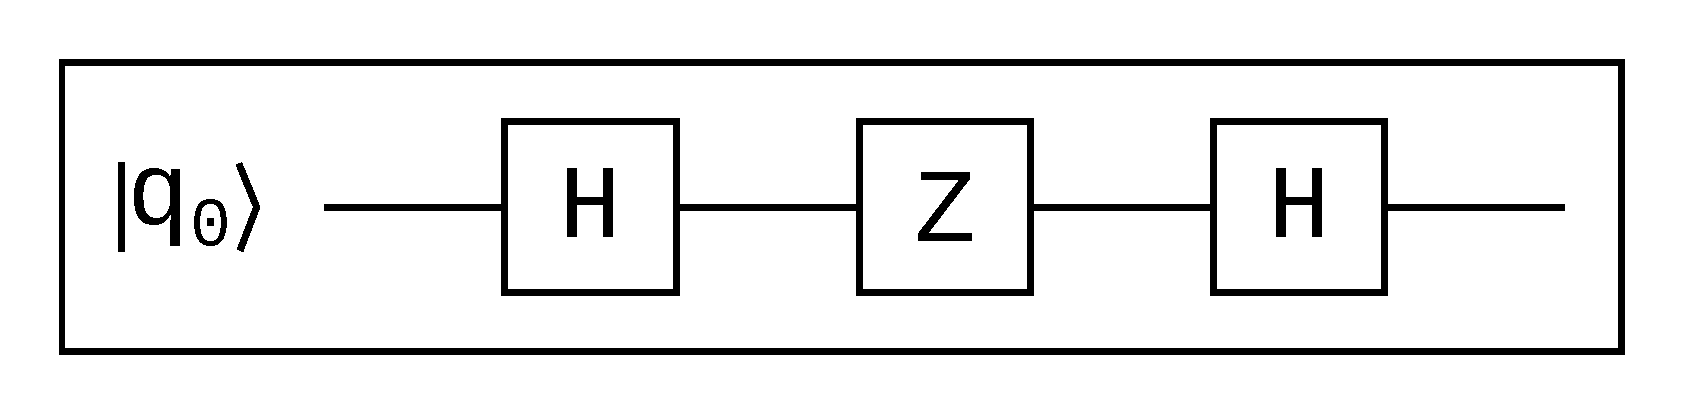
\includegraphics[scale=0.35]{img/qci_a1_question6.ps}}
  \caption{An arbitrary quantum circuit.}
  \label{fig:circuit1}
\end{figure}

\begin{question}
Consider the quantum circuit presented in Figure~\ref{fig:circuit1} and assume $\ket{q_{0}} = \ket{0}$. Determine, by using the Dirac notation, what is the state vector $\ket{\psi_{out}}$?
\label{qst:assignment1_6}
\end{question}
{\small
\texttt{Write down your solution here:}
\begin{equation*}
  \begin{split}
    \ket{0} \\ 
    H &\rightarrow \frac{1}{\sqrt{2}} (\ket{0}+\ket{1})
    \\
    Z &\rightarrow \ket{-} = \frac{1}{\sqrt{2}} (\ket{0}-\ket{1})
    \\
    H &\rightarrow \ket{1}
  \end{split}
\end{equation*}}
\vspace{0.1cm}

\begin{question}
Consider the quantum circuit presented in Figure~\ref{fig:circuit1}. Determine, by using the matrix--matrix multiplication, what is the resulting transformation matrix?
\label{qst:assignment1_7}
\end{question}
{\small
\texttt{Write down your solution here:}

\begin{equation*}
U = H Z H
\end{equation*}

\textbf{Step 1: Defining the Matrix}

\begin{equation*}
H = \frac{1}{\sqrt{2}}
\begin{pmatrix}
1 & 1 \\ 1 & -1
\end{pmatrix}
\end{equation*}

\begin{equation*}
Z = \begin{pmatrix} 1 & 0 \\ 0 & -1
\end{pmatrix}
\end{equation*}

\textbf{Step 2: Compute } ZH

\begin{align*}
ZH &= \begin{pmatrix} 1 & 0 \\ 0 & -1
\end{pmatrix}
\cdot
\frac{1}{\sqrt{2}}
\begin{pmatrix} 1 & 1 \\ 1 & -1
\end{pmatrix} \\
&=
\frac{1}{\sqrt{2}} \begin{pmatrix} 1 & 1 \\ -1 & 1
\end{pmatrix}
\end{align*}

\textbf{Step 3: Compute } H(ZH)

\begin{align*}
U &= \frac{1}{\sqrt{2}} \begin{pmatrix} 1 & 1 \\ 1 & -1
\end{pmatrix}
\cdot
\frac{1}{\sqrt{2}} \begin{pmatrix} 1 & 1 \\ -1 & 1
\end{pmatrix} \\
&=
\frac{1}{2} \begin{pmatrix} 1 & 1 \\ 1 & -1
\end{pmatrix}
\begin{pmatrix} 1 & 1 \\ -1 & 1
\end{pmatrix} \\
&=
\frac{1}{2}
\begin{pmatrix}
(1)(1)+(1)(-1) & (1)(1)+(1)(1) \\
(1)(1)+(-1)(-1) & (1)(1)+(-1)(1)
\end{pmatrix} \\
&=
\frac{1}{2} \begin{pmatrix} 0 & 2 \\ 2 & 0
\end{pmatrix} \\
&=
\begin{pmatrix} 0 & 1 \\ 1 & 0
\end{pmatrix}
\end{align*}

\begin{equation*}
HZH = \begin{pmatrix} 0 & 1 \\ 1 & 0
\end{pmatrix}
= X
\end{equation*}}
\vspace{0.1cm}

\begin{question}
Consider the quantum circuit presented in Figure~\ref{fig:circuit1} and assume $\ket{q_{0}} = \ket{1}$. Determine, by using the matrix--vector multiplication, what is the state vector $\ket{\psi_{out}}$?
\label{qst:assignment1_8}
\end{question}
{\small
\texttt{Write down your solution here:}
\begin{equation*}
  \begin{split}
    &\rightarrow \ket{1} \\
    \textbf{Given: } |q_0\rangle = |1\rangle

\begin{equation*}
|1\rangle =
\begin{pmatrix}
0 \\
1
\end{pmatrix}
\end{equation*}

\textbf{Step 1: Apply the first Hadamard gate } H
\begin{equation*}
H = \frac{1}{\sqrt{2}}
\begin{pmatrix}
1 & 1 \\
1 & -1
\end{pmatrix}
\end{equation*}

\begin{align*}
|\psi_1\rangle
&= H |1\rangle \\
&=
\frac{1}{\sqrt{2}}
\begin{pmatrix}
1 & 1 \\
1 & -1
\end{pmatrix}
\begin{pmatrix}
0 \\
1
\end{pmatrix} \\
&=
\frac{1}{\sqrt{2}}
\begin{pmatrix}
(1)(0) + (1)(1) \\
(1)(0) + (-1)(1)
\end{pmatrix} \\
&=
\frac{1}{\sqrt{2}}
\begin{pmatrix}
1 \\
-1
\end{pmatrix}
\end{align*}

\textbf{Step 2: Apply the Z gate}
\begin{equation*}
Z =
\begin{pmatrix}
1 & 0 \\
0 & -1
\end{pmatrix}
\end{equation*}

\begin{align*}
|\psi_2\rangle
&= Z |\psi_1\rangle \\
&=
\begin{pmatrix}
1 & 0 \\
0 & -1
\end{pmatrix}
\frac{1}{\sqrt{2}}
\begin{pmatrix}
1 \\
-1
\end{pmatrix} \\
&=
\frac{1}{\sqrt{2}}
\begin{pmatrix}
1 \\
1
\end{pmatrix}
\end{align*}

\textbf{Step 3: Apply the final Hadamard gate}

\begin{align*}
|\psi_{out}\rangle
&= H |\psi_2\rangle \\
&=
\frac{1}{\sqrt{2}}
\begin{pmatrix}
1 & 1 \\
1 & -1
\end{pmatrix}
\frac{1}{\sqrt{2}}
\begin{pmatrix}
1 \\
1
\end{pmatrix} \\
&=
\frac{1}{2}
\begin{pmatrix}
(1)(1) + (1)(1) \\
(1)(1) + (-1)(1)
\end{pmatrix} \\
&=
\frac{1}{2}
\begin{pmatrix}
2 \\
0
\end{pmatrix} \\
&=
\begin{pmatrix}
1 \\
0
\end{pmatrix}
\end{align*}

\textbf{Final Result:}

\begin{equation*}
|\psi_{out}\rangle =
\begin{pmatrix}
1 \\
0
\end{pmatrix}
= |0\rangle
\end{equation*}
  \end{split}
\end{equation*}
\vspace{0.1cm}

\begin{figure}[t]
  \centerline{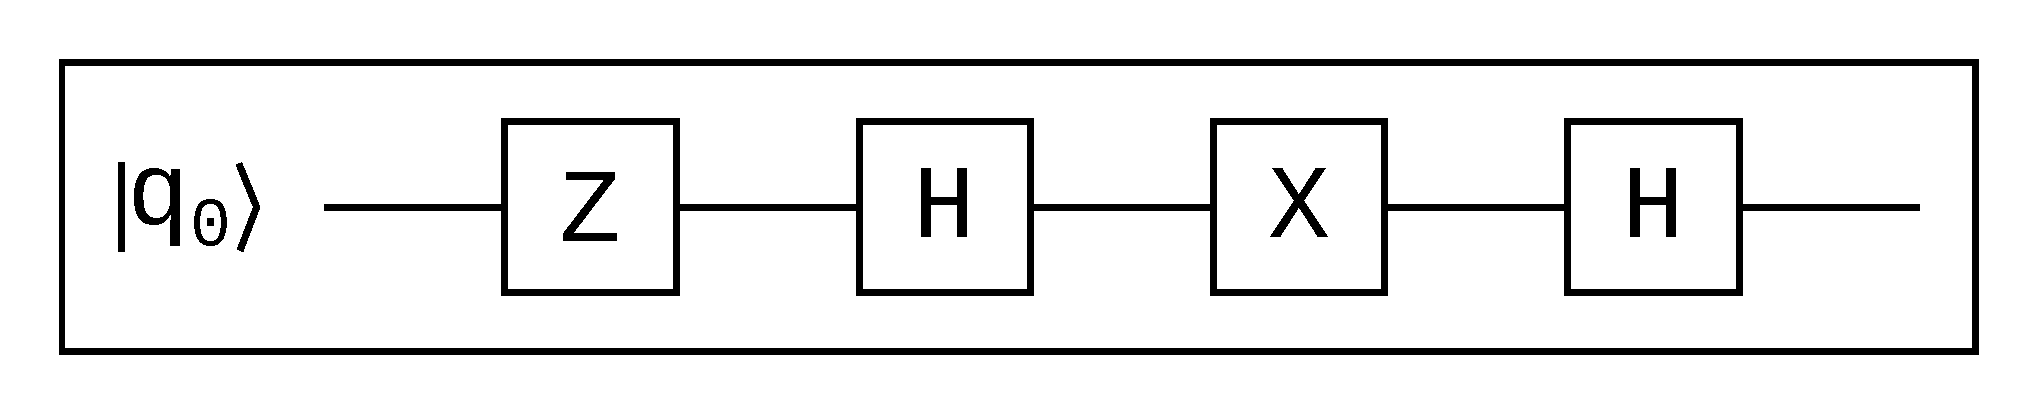
\includegraphics[scale=0.35]{img/qci_a1_question9.ps}}
  \caption{An arbitrary quantum circuit.}
  \label{fig:circuit2}
\end{figure}

\begin{question}
Consider the quantum circuit presented in Figure~\ref{fig:circuit2} and assume $\ket{q_{0}} = \ket{1}$. Determine, by using the Dirac notation, what is the state vector $\ket{\psi_{out}}$?
\label{qst:assignment1_9}
\end{question}
{\small
\texttt{Write down your solution here:}
\begin{equation*}
  \begin{split}
    &\rightarrow \ket{1} \\
    \textbf{Given:}

\begin{equation*}
|q_0\rangle = |1\rangle
\end{equation*}

The circuit is

\begin{equation*}
U = Z H X H
\end{equation*}

\textbf{Step 1: Apply the first } H

\begin{equation*}
H|1\rangle = \frac{1}{\sqrt{2}}(|0\rangle - |1\rangle)
\end{equation*}

\begin{equation*}
|\psi_1\rangle =
\frac{1}{\sqrt{2}}(|0\rangle - |1\rangle)
\end{equation*}

\textbf{Step 2: Apply } X

Using

\begin{equation*}
X|0\rangle = |1\rangle,
\quad
X|1\rangle = |0\rangle
\end{equation*}

\begin{align*}
|\psi_2\rangle
&= X |\psi_1\rangle \\
&=
\frac{1}{\sqrt{2}}(X|0\rangle - X|1\rangle) \\
&=
\frac{1}{\sqrt{2}}(|1\rangle - |0\rangle) \\
&=
-\frac{1}{\sqrt{2}}(|0\rangle - |1\rangle)
\end{align*}

\textbf{Step 3: Apply } H

Using

\begin{equation*}
H|0\rangle = \frac{1}{\sqrt{2}}(|0\rangle + |1\rangle)
\end{equation*}

\begin{equation*}
H|1\rangle = \frac{1}{\sqrt{2}}(|0\rangle - |1\rangle)
\end{equation*}

\begin{align*}
H(|0\rangle - |1\rangle)
&= H|0\rangle - H|1\rangle \\
&=
\frac{1}{\sqrt{2}}(|0\rangle + |1\rangle)
-
\frac{1}{\sqrt{2}}(|0\rangle - |1\rangle) \\
&=
\frac{1}{\sqrt{2}}
\left(
|0\rangle + |1\rangle - |0\rangle + |1\rangle
\right) \\
&=
\sqrt{2} |1\rangle
\end{align*}

Including the prefactor:

\begin{equation*}
|\psi_3\rangle
=
-\frac{1}{\sqrt{2}} \cdot \sqrt{2} |1\rangle
=
- |1\rangle
\end{equation*}

\textbf{Step 4: Apply } Z

\begin{equation*}
Z|1\rangle = -|1\rangle
\end{equation*}

\begin{align*}
|\psi_{out}\rangle
&= Z(-|1\rangle) \\
&= -Z|1\rangle \\
&= -(-|1\rangle) \\
&= |1\rangle
\end{align*}

\textbf{Final Result:}

\begin{equation*}
|\psi_{out}\rangle = |1\rangle
\end{equation*}
  \end{split}
\end{equation*}
\vspace{0.1cm}

\begin{question}
Consider the quantum circuit presented in Figure~\ref{fig:circuit2} and assume $\ket{q_{0}} = \ket{+}$. Determine, by using the Dirac notation, what is the state vector $\ket{\psi_{out}}$?
\label{qst:assignment1_10}
\end{question}
{\small
\texttt{Write down your solution here:}
\begin{equation*}
  \begin{split}
    &\rightarrow \ket{+} \\
    \textbf{Given:}

\begin{equation*}
|q_0\rangle = |+\rangle
=
\frac{1}{\sqrt{2}} (|0\rangle + |1\rangle)
\end{equation*}

The circuit is

\begin{equation*}
U = Z H X H
\end{equation*}

\textbf{Step 1: Apply the first } H

Since

\begin{equation*}
H|+\rangle = |0\rangle
\end{equation*}

we obtain

\begin{equation*}
|\psi_1\rangle = |0\rangle
\end{equation*}

\textbf{Step 2: Apply } X

\begin{equation*}
X|0\rangle = |1\rangle
\end{equation*}

\begin{equation*}
|\psi_2\rangle = |1\rangle
\end{equation*}

\textbf{Step 3: Apply } H

\begin{equation*}
H|1\rangle =
\frac{1}{\sqrt{2}} (|0\rangle - |1\rangle)
\end{equation*}

\begin{equation*}
|\psi_3\rangle =
\frac{1}{\sqrt{2}} (|0\rangle - |1\rangle)
\end{equation*}

\textbf{Step 4: Apply } Z

Since

\begin{equation*}
Z|0\rangle = |0\rangle,
\quad
Z|1\rangle = -|1\rangle
\end{equation*}

we get

\begin{align*}
|\psi_{out}\rangle
&= Z |\psi_3\rangle \\
&=
\frac{1}{\sqrt{2}} (Z|0\rangle - Z|1\rangle) \\
&=
\frac{1}{\sqrt{2}} (|0\rangle + |1\rangle)
\end{align*}

\textbf{Final Result:}

\begin{equation*}
|\psi_{out}\rangle =
\frac{1}{\sqrt{2}} (|0\rangle + |1\rangle)
=
|+\rangle
\end{equation*}
  \end{split}
\end{equation*}
